%!TEX root = ../agi_mfwis415af4l.tex
\section{Beschreibung des Projektverlaufs}
\label{concept}

\subsection{Tatsächliche Aufgabenverteilung im Team}
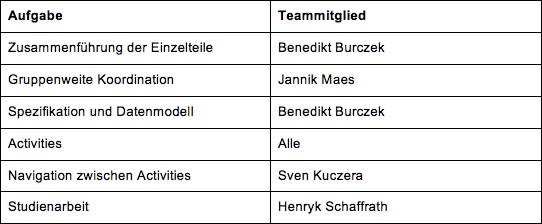
\includegraphics[scale=0.8]{img/geplanteAugabenVerteilung}
\subsection{Teammeetingprotokolle}\\
\\
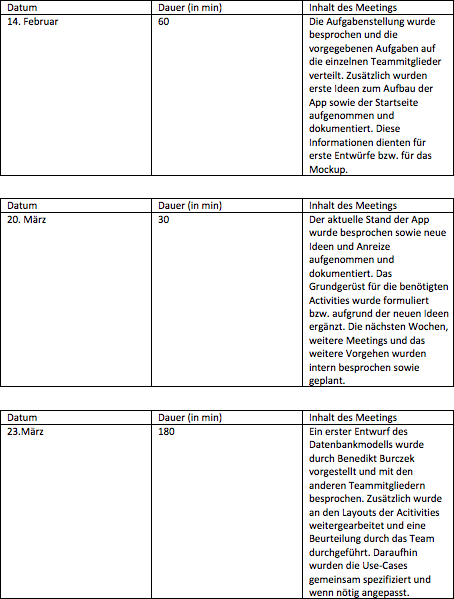
\includegraphics[scale=1]{img/PTB1.png}\\
\\
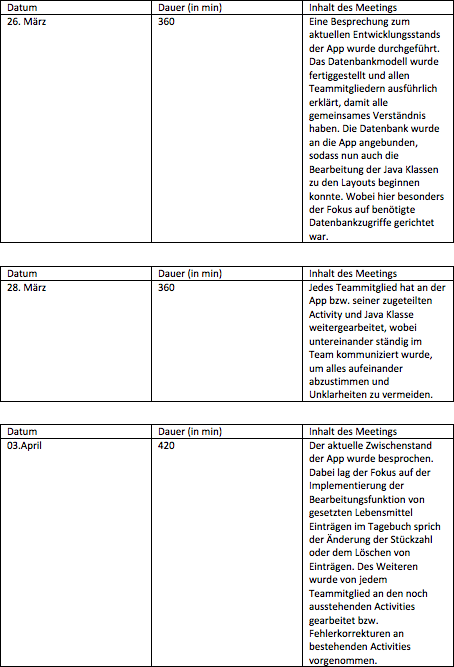
\includegraphics[scale=1]{img/PTB2.png}\\
\\
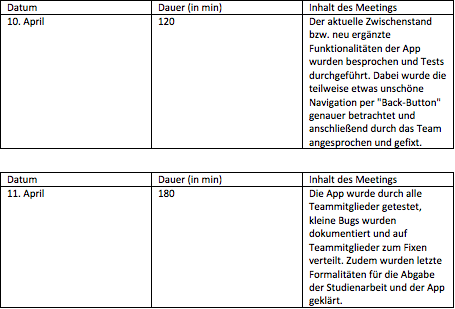
\includegraphics[scale=1]{img/PTB3.png}\\
\\
\subsection{Projekttagebücher aller Teammitglieder}

\subsection{Beschreibung von Problemen}
\textbf{Known Bugs}\\

\begin{itemize}
\item Bei einem Eintrag im Kalorientagebuch kann die Einheit nicht mehr geändert werden.
\item Das Kopieren eines Eintrags ist noch nicht möglich, allerdings können diese verschoben werden.
\item Mengenangaben bei Menüs noch nicht möglich
\item Beim Löschen eines Lebensmittels bleiben Menüs noch nicht unberührt
\item Das Löschen von Entsprechungen und das Erhaltenbleiben einer Mindestangabe ist noch nicht möglich
\item Die Änderung einer Entsprechung passt bisher nur im Tagebuch automatisch die Kalorienanzahl an
\item Kalorientagebucheinträge mit Menüs können noch nicht vollständig, gemäß den Anforderungen, beim Bearbeiten angezeigt werden. Die Daten sind jedoch ordnungsgemäß in der Datenbank hinterlegt
\end{itemize}\\

\textbf{Umstände im Projekt}\\

Die größten Umstände im Projektverlauf waren vor allem zum einen der mangelnden Zeit, durch die Belegung von Terminen durch Klausuren und Vorträge/Ausarbeitungen bei anderen Kursen und durch Hardware/Software Probleme gegeben.\\
Das Projekt hat sich zeitlich genau in die Klausurphase gelegt, wodurch ein stetiges konzentriertes Arbeiten ohne Unterbrechungen und Pause leider nicht möglich war. Das ist der Grund warum viel Zeit für die Planung benötigt wurde. Die verschiedenen Teammitglieder hatten unterschiedliche Projekte und Klausuren, zu diversen Terminen. In dem Projekt 
\textit{food4life}
wurden daher viele Teammeetings gehalten, damit Fragen und Weiteres sofort geklärt werden konnten, damit ein Einhalten des Terminplanes, trotz einer straffen Struktur dennoch möglich ist. Außerdem standen noch diverse andere Termine der FHDW dem Zeitmanagement eher kritisch gegenüber.\\
Ein weiteres großes Problem waren Hard- und Software Probleme, der Android Studio Emulator hat in den besten Fällen schlecht funktioniert, meistens aber gar nicht. Ein erfolgreiches, ununterbrochenes Entwickeln war daher kaum möglich. Das Zurückgreifen auf alternative physische Android Geräte war beschränkt. Verschiedene Unstimmigkeiten in unterschiedlichen Versionen von Android Studio brachten das Projekt auch häufig zu einem kurzen Stopp für mehrere Teammitglieder.
